% !BIB TS-program = biber
\documentclass{frontiersSCNS} % for Science articles



\usepackage{graphicx}
%
\usepackage{amsmath} 
\usepackage{mathptmx}      % use Times fonts if available on your TeX system
%
\usepackage{color, soul}

\usepackage{caption}
\usepackage{float}
\floatstyle{plaintop}

\usepackage{hyperref}

% bibliography
\usepackage[english]{babel}
\usepackage{csquotes}
\usepackage[
backend=biber, 
bibencoding=utf8, 
style=authoryear, 
date=year, 
maxbibnames=6, 
minbibnames=6, 
url=false, 
isbn=false, 
eprint=false,
uniquename = false, 
autocite=inline]{biblatex}
\addbibresource{Bibliography.bib}

\usepackage[draft, nomargin, marginclue, footnote]{fixme}
\fxsetup{targetlayout=color}

% new commands and shortcuts
\usepackage{xspace}
\newcommand{\eg}{\textit{e.g.}\xspace}
\newcommand{\etal}{\textit{et al.}\xspace}
\newcommand{\ie}{\textit{i.e.}\xspace}
\newcommand{\etc}{\textit{etc.}\xspace}
\newcommand{\vs}{\textit{vs.}\xspace}
\newcommand{\viz}{\textit{viz.}\xspace}

% shortcut for float placing
\usepackage{placeins}

% make pretty MATLAB code
\usepackage{listings}
\usepackage{matlab-prettifier}
\lstMakeShortInline[style=Matlab-editor]"

% other nice features
\usepackage{lineno}
\linenumbers

\usepackage{xifthen}% provides \isempty test

\copyrightyear{}
\pubyear{}

\def\journal{Neuroinformatics}
\def\DOI{}
\def\articleType{Technology Report}
\def\keyFont{\fontsize{8}{11}\helveticabold }
\def\firstAuthorLast{Hoyland {et~al.}} 
\def\Authors{Srinivas Gorur-Shandilya\,$^{1*\dagger}$, Alec Hoyland\,$^{1\dagger}$, and Eve Marder$^{1}$}
\def\Address{$^{1}$Volen Center and Biology Department \\ Brandeis University \\ Waltham, MA 02453 \\ USA
\vspace{0.25cm}

\vspace{0.5em}\tiny{$\dagger$ These authors have equally contributed to this article.}
}
\def\corrAuthor{Srinivas Gorur-Shandilya \vspace{1mm}}
%\def\corrAddress{Marder Lab, Brandeis University, Biology Department and Volen Center for Complex Systems, Waltham, MA, USA}
\def\corrAddress{Volen Center for Complex Systems, Brandeis University, Waltham MA 02453}
\def\corrEmail{\texttt{srinivasgs@brandeis.edu}}

\begin{document}
\onecolumn
\firstpage{1}

\title[xolotl: neuron \& network simulator]{Xolotl: An Intuitive and Approachable Neuron \& Network Simulator in MATLAB}
\author[\firstAuthorLast ]{\Authors}
\address{}
\correspondance{}
\extraAuth{}
\topic{An Intuitive Neuronal Simulator}

\maketitle

\begin{abstract}
	
	Information processing by neurons relies on the transmission and interaction of electrical signals that arise from the biophysics of ion channels and synapses. Electrophysiological characterization of these mechanisms has allowed for the construction of conductance-based models that can reproduce many features of neuronal and circuit behavior. However, working with conductance-based models continues to be a challenge due to their high dimensionality, hindering intuition of their dynamical features. Here, we present a neuron and network simulator built on a novel automatic type system that binds class templates written in "C++" to object-oriented code in "MATLAB". Our approach combines the speed and powerful features of "C++" code with the ease-of-use and rich libraries of scientific programming languages like "MATLAB". In our software, models are hierarchical, and components are named and searchable, permitting high-level programmatic control over all parameters. The simulator's architecture allows for the live manipulation of any parameter in any model, and for visualizing the effects of changing that parameter on model behavior. The simulator is fully featured with hundreds of ion channel models from the electrophysiological literature, and can be easily extended to include arbitrary mechanisms and dynamics. Finally, the simulator is written in a modular fashion and has been released under a permissive free software license, enabling it to be integrated easily in third party applications.
	
	\tiny
	\keyFont{ \section{Keywords:} simulator, MATLAB, C++, conductance-based, neuron, network, pedagogy}
	
\end{abstract}

%%%%%%%%%%%%%%%%%%%%%%%%%%%%%%%%%%%%%%%%%%%%%%%%%%%%%%%%%%%%%%%%%%%%%%%%%
%
%
%
%		INTRODUCTION & OVERVIEW
%
%
%
%%%%%%%%%%%%%%%%%%%%%%%%%%%%%%%%%%%%%%%%%%%%%%%%%%%%%%%%%%%%%%%%%%%%%%%%%


\section{Introduction}
\label{sec:intro}

Nervous systems process and transmit information using electrically excitable membranes. Conductance-based models are powerful biophysical simplification of an electrically excitable cell (\cite{hodgkinQuantitativeDescriptionMembrane1952}). Studies based on the Hodgkin-Huxley formalism now contribute significantly to mainstream research in small-circuit networks (\cite{marderTheoryMotion1995, prinzComputationalApproachesNeuronal2010, prinzInsightsModelsRhythmic2006}). Additionally, these models provide an approachable framework for understanding salient principles of neuroscience. However, several challenges remain in simulating biophysically-detailed conductance-based neuron models. First, these models can be high-dimensional with many nonlinear differential equations, with several parameters. Second, many or all equations are strongly coupled through the variables like the membrane potential, and in multi-compartment models, all membrane potentials and their equations are coupled to each other. Finally, the choice of programming language imposes tradeoffs in neuron and network simulators: simulators written in languages like "C", "C++", or "hoc" can integrate equations quickly, but often lack the ease-of-use and interoperability of those written in scientific programming languages like "Python", "Julia" or "MATLAB". 

Two major approaches have dominated the design of neuron simulators. First, some simulators, such as "NEURON" (\cite{hinesNEURONSimulationEnvironment1997}) use a custom language to specify modular network components. These simulators tend to perform fast computations with little overhead, but suffer from a steep learning curve. Wrapping "NEURON" in a more approachable language like "Python" and use of graphical interfaces mitigate these drawbacks, at the cost of obfuscating the underlying algorithms and parameters (\cite{bretteSimulationNetworksSpiking2007, hinesNEURONPython2009}). In contrast, many simulators have been designed to be used entirely in popular scientific programming languages. These simulators can be easier to use, and can benefit from inter-compatibility with other tools. Programs like "DynaSim" (\cite{sherfeyDynaSimMATLABToolbox2018}), "ANNarchy" (\cite{vitayANNarchyCodeGeneration2015}), "BRIAN" (\cite{stimbergBrianSecondComing2013}) allow the user to specify models using strings of equations that are specified in the scientific programming language, that can be translated into a faster implementation language such as "C" or "C++" (\cite{stimbergEquationorientedSpecificationNeural2014}). This approach permits considerable flexibility for simulating systems of differential equations, but the syntax tends to be verbose and the hierarchical nature of conductance-based neuron models is not naturally reflected in the constructed model. Neither approach permits tools that simultaneously maintain efficiency, ease-of-use, and clarity.

To overcome these design limitations, we have developed a novel automatic type system, "cpplab", which binds "MATLAB" code to "C++" header files. This architecture automatically creates objects in "MATLAB" that represent the underlying object-oriented "C++" code, without having to re-specify these objects in "MATLAB". In this paper, we introduce "xolotl", an implementation of the "cpplab" system specialized in integrating conductance-based neuron and network models. Models can be easily constructed from network building blocks in a few lines of "MATLAB" code using a hierarchical and intuitive syntax. Since model objects in the "MATLAB" workspace are automatically linked to the "C++" specification, configuring these objects in "MATLAB" transparently configures the underlying "C++" objects. "xolotl" comes packaged with hundreds of conductances and synapses, built-in visualization functions, and a graphical user interface (GUI) for real-time manipulation of model parameters. Plotting of voltage, intracellular calcium, conductance gating functions, and time constants is provided by built-in "xolotl" methods. The GUI permits real-time tuning of any network parameters using numerical sliders in a graphical interface which displays the resultant membrane potential and intracellular calcium traces. The ease-of-use of these tools lends them to pedagogical applications and rapid exploration of toy models. This tool aims to simplify the investigation of dynamics of biophysically-realistic network models, facilitate collaborative modeling, and complement other tools being developed in the computational neuroscience community.

%%%%%%%%%%%%%%%%%%%%%%%%%%%%%%%%%%%%%%%%%%%%%%%%%%%%%%%%%%%%%%%%%%%%%%%%%
%
%
%
%		DESIGN GOALS
%
%
%
%%%%%%%%%%%%%%%%%%%%%%%%%%%%%%%%%%%%%%%%%%%%%%%%%%%%%%%%%%%%%%%%%%%%%%%%%

\section{Design Goals}
\label{design}

"xolotl" is designed to be easy-to-use and richly featured and that is fast enough to use in everyday research. Our focus was on designing a simulator of conductance-based neurons and networks of these neurons; and simulating arbitrary dynamical systems is therefore beyond the scope of this software. The software is designed to be used from within "MATLAB", a scientific programming language popular amongst neuroscientists and engineers for pedagogy and research. Our goal is to make "xolotl" completely usable entirely within MATLAB, and all parameters of models can be be inspected and edited before running the model. Several features of the simulator are designed to be easily extensible, and the simulator appears in the "MATLAB" workspace as a first-class native object, and is fully compatible with the large library of toolboxes that a scientific programming environment like "MATLAB" provides. 

\subsection{Features}
\label{features}

\paragraph{A rich library of network components.} "xolotl" comes packaged with hundreds of pre-existing components (compartments, synapses, conductances, and controllers) which are used to construct model neurons and networks. Compartments represent cylindrical sections of membrane with a single membrane potential, and can represent either entire cells or parts of cells. Synapses connect two compartments together by introducing a current in the post-synaptic neuron that depends on the voltage of the presynaptic neuron. Conductances represent populations of ion channels in a compartment that produce transmembrane currents. Controllers represent homeostatic mechanisms that integrate a Calcium-dependent signal from the compartment they are in and  change the properties of a conductance or synapse in response.

\paragraph{Object-oriented.}
"xolotl" is designed to mirror the nested and hierarchical structure of networks and neurons.  Biological neuronal networks consist of neurons that are connected to each other with synapses. Each of these neurons contains within it a set of conductances and synaptic currents that affect its electrical behavior. Similarly, a "xolotl" model can contain a set of compartments that can represent individual neurons. Each compartment can contain a set of conductances. All objects in the "xolotl" model tree (compartments, conductances, etc.) are bonafide "MATLAB" objects that have their own type, properties and associated methods. This object-oriented programming paradigm naturally represents the hierarchical structure of biological neurons and networks. 

\paragraph{Automatic type system.}
When a network component is added in "MATLAB", the "xolotl" structure is updated, and "cpplab" automatically constructs and compiles the "C++" from the requisite header files. "MATLAB" treats "cpplab" constructions as fully-typed first-class objects allowing for symbolic manipulation using only the high-level programming language and graphical interfaces. "xolotl" simulations are run entirely from "C++" executables; the inputs and outputs can be represented entirely in "MATLAB".

\paragraph{Automatic compiling.}
The user experience of "xolotl" can stay entirely in "MATLAB". Transpiling and compiling of "C++" is performed automatically. Cryptographic hashing of the "xolotl" object confirms that compiling occurs only when necessary, and that the correct binary is used during integration.

\subsection{Limitations}
\label{limitations}

The focus on ease-of-use and fast simulations means some features were intentionally neglected in the design process. 

\paragraph{Limited to conductance-based models.} "xolotl" has been developed specifically for conductance-based models. It does not currently support rate- or current-based models, or arbitrary dynamical systems. 

\paragraph{Limited numerical integration strategies.} While the exponential Euler method performs well in neuronal models (\cite{ohErrorAnalysisSpecialized2006, dayanTheoreticalNeuroscience2001}, it may be desirable to use other methods under certain conditions. "xolotl" does not currently support other integration schemes for its built-in conductances, nor does the software support error-sensitive variable step-sizes `out-of-the-box.'

\paragraph{Inefficient tools for handling large networks.} While "xolotl" can integrate large networks ($>1000$ compartments), "xolotl" uses string-based comprehension for labeling compartments which is suited to descriptive naming, but prohibits vector operations over compartments.

\paragraph{New mechanisms require new \texttt{C++} code.} Adding new network components also requires writing some "C++" code. Adding a new conductance in the Hodgkin-Huxley formalism (\cite{hodgkinMeasurementCurrentvoltageRelations1952, dayanTheoreticalNeuroscience2001}), requires creating a new "C++" header file, though this is generally trivial. Implementing a new integration scheme or "cpplab" class requires much more in-depth knowledge of "C++" and modification of the core code.

%%%%%%%%%%%%%%%%%%%%%%%%%%%%%%%%%%%%%%%%%%%%%%%%%%%%%%%%%%%%%%%%%%
%
%
%
%		USAGE EXAMPLES
%
%
%
%%%%%%%%%%%%%%%%%%%%%%%%%%%%%%%%%%%%%%%%%%%%%%%%%%%%%%%%%%%%%%%%%%

\section{Usage Examples}
\label{usage}

In this section, we illustrate how "xolotl" can be used to generate a variety of models and simulate them. These examples have been chosen to illustrate various features of "xolotl", and are intended to serve as a template that researchers and educators can use for their own needs. 

%%%%%%%%%%%%%%%%%%%%%%%%%%%%%%%%%%%%%%%%%%%%%%%%%%%%%%%%%%%%%%%%%%
%
%
%
%		SIMULATING A HODGKIN-HUXLEY MODEL
%
%
%
%%%%%%%%%%%%%%%%%%%%%%%%%%%%%%%%%%%%%%%%%%%%%%%%%%%%%%%%%%%%%%%%%%

\subsection{Simulating a Hodgkin-Huxley Model}

The axon of the giant squid contains contains a fast inactivating sodium conductance ("NaV"), a slower non-inactivating potassium conductance ("Kd"), and a passive leak current. Seminal work by Hodgkin and Huxley showed that depolarizations of the membrane, for example, by injecting current, could lead to an activation of the voltage-sensitive "NaV" channels, which led to a run away depolarization that was terminated by the inactivation of "NaV" channels and the activation of "Kd" channels that repolarized the membrane (\cite{hodgkinComponentsMembraneConductance1952, hodgkinMeasurementCurrentvoltageRelations1952}). The Hodgkin-Huxley model generates action potentials, and, as one of the simplest models of excitable neural mebranes, often serves as a the first model introduced in pedagogical literature (cite some textbooks).  


\begin{figure}
	\centering
	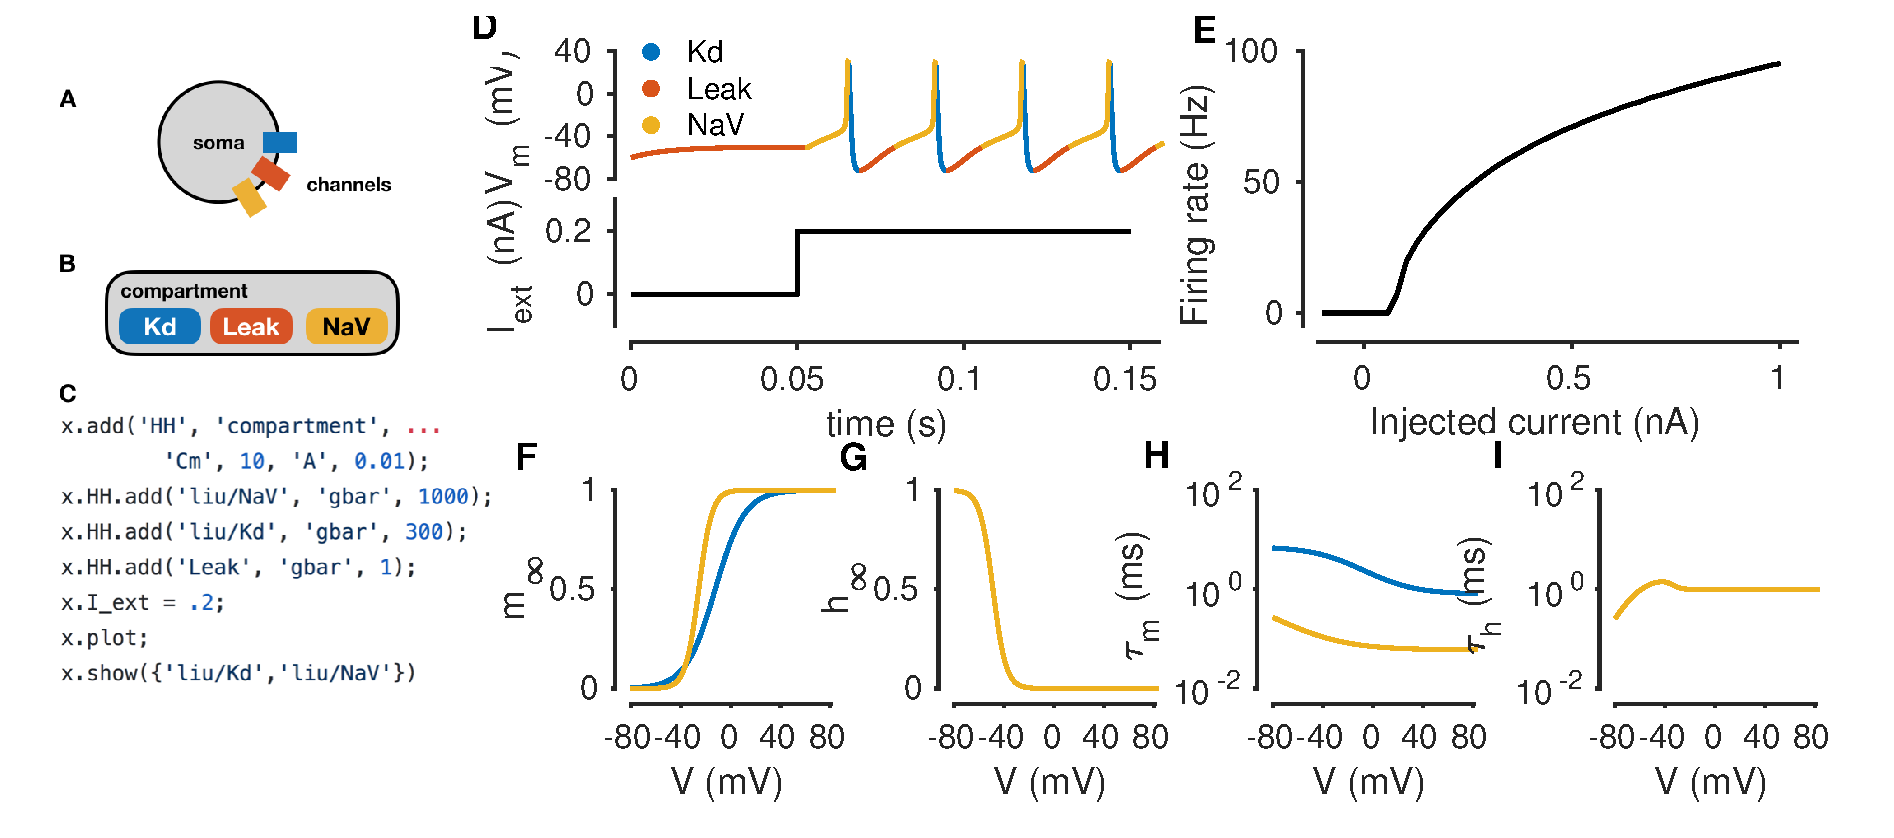
\includegraphics[width=1.0\linewidth]{gfx/figure_HH}
	\caption{\texttt{xolotl} can quickly set up and simulate conductance-based models. Schematic representation of a electrotonically-neuron with three populations of ion channels (colored rectangles). In the simulator, the soma is represented using ab object of class $compartment$ and the populations of ion channels are represented by $conductance$ objects contained within the compartment. Code snippet used to set up this neuron model, inject current, integrate and plot the voltage, and show activation functions demonstrates how various several steps can be run in a few lines of code. (A) Simulated voltage trace of a Hodgkin-Huxley model with three conductances and 0.2 nA of injected current. Colors indicate the dominant current (gold is fast sodium (NaV), blue is delayed rectifier (Kd), red is Leak). (C) f-I curve of this neuron. (D-E) Steady-state gating functions for activation (m) and inactivation (h) gating variables. (F-I) Voltage-dependence of time constants for activation (m) and inactivation (h) gating variables}
	\label{fig:figurehh}
\end{figure}

In this section, we demonstrate how to simulate a Hodgkin-Huxley-like model, and how the tools built into our simulator make it easy to set up and integrate the model, and gain insight into the underlying biophysical mechanism. The schematic in Figure \ref{fig:figurehh} shows how the hierarchical structure of the ion channel populations within the soma is represented in the simulator, and how to create a compartment (here, labelled "HH") and add three populations of ion channels to it. These models of ion channels were obtained from \cite{liuModelNeuronActivitydependent1998} based on electrophysiological recordings from the lobster stomatogastric ganglion (\cite{turrigianoSelectiveRegulationCurrent1995}), and are part of the simulator. Adding an injected current and calling the built-in "plot" function plots the time series of membrane voltage. In the absence of injected current, the model is quiescent. When 0.2 nA is injected, the model tonically spikes (Figure \ref{fig:figurehh}A-B).  The \texttt{plot} function generates a voltage trace, which is colored by the dominant current (Figure \ref{fig:figurehh}A). If the membrane potential is increasing, the strongest instantaneous inward current colors the trace. Conversely, if the membrane potential is decreasing, the strongest outward current colors the trace instead. These built-in features reveal that the dominant current during the upswing of every action potential is the sodium current, and the dominant current immediately after the peak of the action potential is the potassium current. This feature could be useful in quickly understanding the contributions of a number of ion channel types in a complex voltage trace from a more complicated neuron model. 

The model can be integrated for various amplitudes of injected current to determine its f-I curve, or the relationship between injected current and its firing rate (cite). Figure \ref{fig:figurehh}C shows the f-I curve of this model, obtained by repeated integration of the model.  Finally, the built-in \texttt{show} function can plot activation (m) and inactivation (h) curves and voltage-dependent timescales of any channel type in the simulator (Figure \ref{fig:figurehh}D-G). These plots revleal that activation kinetics of the "NaV" channels are much faster than that of the "Kd" channels (Figure \ref{fig:figurehh}F), which facilitates the transient depolarization in an action potential. In summary, the simulator allows the user to construct and integrate this model in a few lines of code, and provides a rich visualization of the dynamics of the model. 


%%%%%%%%%%%%%%%%%%%%%%%%%%%%%%%%%%%%%%%%%%%%%%%%%%%%%%%%%%%%%%%%%
%
%
%
%		VOLTAGE CLAMP
%
%
%
%%%%%%%%%%%%%%%%%%%%%%%%%%%%%%%%%%%%%%%%%%%%%%%%%%%%%%%%%%%%%%%%%

\subsection{Performing a Voltage Clamp Experiment \textit{in-silico}}

"xolotl" can recapitulate the results of voltage clamp experiments (\cite{turrigianoSelectiveRegulationCurrent1995, swensenMultiplePeptidesConverge2000, swensenModulatorsConvergentCellular2001, destexheDynamicClampPrinciplesApplications2009}). Figure \ref{fig:figureclamp} displays steps in the procedure to clamp the membrane potential of a cell with delayed rectifier potassium conductance. During an \textit{in-vitro} experiment, confounding currents would be pharmacologically-blocked and two-electrode voltage clamp used to record tail currents at fixed membrane potential (\cite{connorInwardDelayedOutward1971, connorVoltageClampStudies1971}).

A single-compartment model with a delayed-rectifier conductance (\cite{liuModelNeuronActivitydependent1998}) is simulated at stepped membrane potentials. The "integrate" function outputs the membrane potential and current as time series. Currents under voltage clamp approach the steady-state holding current (Figure \ref{fig:figureclamp}D-E). The current-voltage relation is the steady-state current over the clamped voltage, and the effective conductance is the derivative of that relation (Figure \ref{fig:figureclamp}F-G). Since the effective conductance is the product of the maximal conductance and the gating variables (\cite{dayanTheoreticalNeuroscience2001, turrigianoSelectiveRegulationCurrent1995}) and the tail current is monotonically-increasing with time under voltage clamp, the current can be represented as non-inactivating. Fitting a sigmoid to various powers yields a model for the current dynamics (Figure \ref{fig:figureclamp}H-I). These figures describe graphically the theoretical underpinnings of current analysis through voltage clamp and can serve as an effective pedagogical tool for computational and quantitative neuroscience.

%%%%%%%%%%%%%%%%%%%%%%%%%%%%%%%%%%%%%%%%%%%%%%%%%%%%%%%%%%%%%%%%%
%
%
%
%		NETWORK MODELS
%
%
%
%%%%%%%%%%%%%%%%%%%%%%%%%%%%%%%%%%%%%%%%%%%%%%%%%%%%%%%%%%%%%%%%%

\subsection{Simulating Network Models}

Network models in "xolotl" consist of compartment objects connected by synapses. Presynaptic and postsynaptic labels indicate the connectivity of the synapse. Figure \ref{fig:figurenetwork} implements a model of the triphasic pyloric rhythm in the stomatogastric ganglion of crustaceans (\cite{prinzSimilarNetworkActivity2004}). The pyloric model contains three compartments and seven synapses (Figure \ref{fig:figurenetwork}A). This structure is recapitulated in the hierarchy of the "xolotl" object, where conductances are contained within compartments (Figure \ref{fig:figurenetwork}B). Synapses are stored in a vector array as a field of the "xolotl" object in "MATLAB" (Figure \ref{fig:figurenetwork}C).

%%%%%%%%%%%%%%%%%%%%%%%%%%%%%%%%%%%%%%%%%%%%%%%%%%%%%%%%%%%%%%%%%%%%%%%%%
%
%
%
%		INTEGRAL CONTROL
%
%
%
%%%%%%%%%%%%%%%%%%%%%%%%%%%%%%%%%%%%%%%%%%%%%%%%%%%%%%%%%%%%%%%%%%%%%%%%%

\subsection{Simulating Homeostasis}

"xolotl" can implement homeostatic tuning rules as integral control. The controller computes an error signal (typically a function of intracellular calcium concentration), and adjusts the conductance or synapse it controls accordingly (\cite{olearyCorrelationsIonChannel2013}). In "xolotl", integral controllers are "cpplab" objects added to the conductance or synapse they regulate.

In a demonstration adapted from \cite{olearyCorrelationsIonChannel2013}, integral control changes maximal conductances to bring a neuron from quiescence into a bursting regime. Calcium sensors supervene on maximal conductance density (Figure \ref{fig:figureintegralcontrol}) to change neuronal activity. Each conductance in the "xolotl" structure contains a calcium-sensitive controller (Figure \ref{fig:figureintegralcontrol}B-C). Maximal conductances increase from random initial conditions to a set which elicits the desired network output by minimizing the error signal (Figure \ref{fig:figureintegralcontrol}D-F).

%%%%%%%%%%%%%%%%%%%%%%%%%%%%%%%%%%%%%%%%%%%%%%%%%%%%%%%%%%%%%%%%%%%%%%%%%
%
%
%
%		GRAPHICAL INTERFACE
%
%
%
%%%%%%%%%%%%%%%%%%%%%%%%%%%%%%%%%%%%%%%%%%%%%%%%%%%%%%%%%%%%%%%%%%%%%%%%%

\subsection{Using the GUI to manipulate parameters}

The "manipulate" function opens the GUI which permits visualization of changing parameters in real-time. Moving sliders representing the values of network parameters updates a plot (Figure \ref{fig:puppeteerscreenshot}B). By default, the function opens a figure displaying the results of the "plot" function, which shows the voltage and intracellular calcium traces for each compartment (Figure \ref{fig:puppeteerscreenshot}A). "manipulate" grants slider control over all "xolotl" parameters by default, but specific ones can be selected by passing them as arguments.


%In "MATLAB", users create a "xolotl" object and populate it with "cpplab"-generated objects which describe compartments, conductances, synapses, and controllers. The model is integrated with the "integrate" function where the membrane potential, intracellular calcium concentration, controller states, intrinsic currents, and synaptic currents can be outputs.
%
%
%
%\subsection{Constructing Networks}
%
%The "add" function creates a compartment, conductance, or controller and affixes it as a field in the "xolotl" network structure. This function generates a "MATLAB struct" that faithfully represents the underlying "C++" code. Compartments add to the "xolotl" object and conductances add to compartments. Specific properties can be specified using key-value pair arguments (\eg Figure \ref{fig:figurehh}A).
%
%\paragraph{Compartments.}
%A model neuron consists of one or more compartments, each representing a section of membrane with capacitance and surface area. Isopotential models require one compartment, whereas models with multiple neurons, units, or non-trivial morphology require multiple compartments.
%
%%\begin{table}
%%	\begin{center}
%%		\begin{tabular}{ l | l | c }
%%			\textbf{Name} & \textbf{\texttt{PropertyName}} & Units \\ \hline
%%			Membrane potential & "V" & $mV$ \\
%%			Intracellular calcium concentration & "Ca" & $\mu M$ \\
%%			Membrane capacitance & "Cm" & $nF/mm^2$ \\
%%			Volume & "vol" & $mm^3$ \\
%%			Surface area & "A" & $mm^2$ \\
%%			Radius of compartment & "radius" & $mm$ \\
%%			Length of compartment & "len" & $mm$ \\
%%			Extracellular calcium steady-state & "Ca_out" & $\mu M$ \\
%%			Intracellular calcium steady-state & "Ca_in" & $\mu M$ \\
%%			Calcium buffering shell thickness & "shell_thickness" & $\mu M$ \\
%%			Calcium current to concentration factor & "phi" & ??? \\
%%			Calcium buffering time constant & "tau_Ca" & $ms$ \\
%%			Average calcium concentration & "Ca_average" & $\mu M$ \\
%%			Target calcium concentration & "Ca_target" & $\mu M$ \\
%%		\end{tabular}
%%	\end{center}
%%	\label{tab:compartmentprops}
%%\end{table}
%
%\paragraph{Synapses.}
%"xolotl" provides some features for generating complex models. Synapses can be added with the \texttt{connect} function. Synapses possess identifiers to presynaptic and postsynaptic compartments and default to electrical synapses. To create axons or transport chains, the \texttt{slice} function splits a compartment into $n$ discrete segments and adds these compartments to the network connected by electrical synapses.
%
%%\begin{center}
%%	\begin{tabular}{ l | l | c }
%%		\label{tab:synapseprops}
%%		\textbf{Name} & \textbf{\texttt{PropertyName}} & Units \\ \hline
%%		Maximal conductance & "gbar" & $\mu S /mm^2$ \\
%%		Reversal potential & "E" & $mV$ \\
%%		Synaptic gating variable & "s" &  \\
%%	\end{tabular}
%%\end{center}
%
%\paragraph{Conductances and controllers.}
%
%All conductances contain fields for maximal conductance and reversal potential. Conductances with activation and inactivation variables include them as $m$ and $h$ respectively. Gating functions and their respective time constants are contained within the conductance header file. "xolotl" comes packaged with conductances from several dozen papers (\cite{dethierPositiveFeedbackCellular2015}.
%
%%\begin{center}
%%	\begin{tabular}{ l | l | c }
%%		\textbf{Name} & \textbf{\texttt{PropertyName}} & Units \\ \hline
%%		Maximal conductance & "gbar" & $\mu S /mm^2$ \\
%%		Reversal potential & "E" & $mV$ \\
%%		Activation gating variable & "m" &  \\
%%		Inactivation gating variable & "h" &  \\
%%	\end{tabular}
%%\end{center}
%
%\paragraph{Creating custom \texttt{cpplab} objects.}
%
%"xolotl" contains template header files for producing custom conductances. The template contains instructions on how to design novel conductances with arbitrary specifications.
%
%\subsection{Simulation}
%
%Models are simulated in "xolotl" with the \texttt{integrate} function which outputs as time series the membrane potentials, intracellular calcium concentrations, controller states, intrinsic currents, and synaptic currents. The \texttt{integrate} function also accepts an argument which specifies injected current or clamped voltage. 
%
%\paragraph{Numerical integration.}
%"xolotl" uses the exponential Euler method for single compartment models, forward Euler for gating variables, and a Crank-Nicholson regime for electrically-coupled compartments (\cite{ohErrorAnalysisSpecialized2006, dayanTheoreticalNeuroscience2001, butcherNumericalDifferentialEquation2016}). These defaults provide a mix of speed, accuracy, and stability, and are built into the "cpplab" header files. Custom "cpplab" header files can be customized with any iterative integration method. The simulation time-resolution can be specified to target arbitrary precision, and an output time step can be selected to support automatic down-sampling for memory considerations.
%
%\paragraph{`Closed-loop' vs. `open-loop.'}
%Simulations can be run in `closed-loop' mode where each simulation begins by resetting all dynamical variables to their initial conditions at instantiation, or `open-loop' mode which begins simulation with the current network state.
%
%\subsection{Additional Features}
%
%\paragraph{Using the graphical interface to manipulate parameters.}
%
%"xolotl" comes packaged with a graphical user interface for visualizing parameter changes in real-time. The \texttt{manipulate} function opens the GUI, which displays a figure plotting the membrane potential and intracellular calcium concentration of all compartments as time series, and a dialog box with customizable sliders for all parameters of the model, much like the "Manipulate" function in Wolfram "Mathematica". Moving the sliders integrates the model in `open-loop` mode with the new parameters. Closing the GUI saves the network state of the model to the "xolotl" object. This is particularly helpful for rapid prototyping of models.
%
%\paragraph{Optimizing parameters.}
%"xolotl" can use the Global Optimization toolbox for "MATLAB" to optimize any accessible "xolotl" parameters. The toolbox is algorithm-agnostic and accepts any function in "MATLAB" with a scalar first output as the objective function. Simulations run on multi-core processors or high-performance computing clusters using the Parallel Computing toolbox.

%%%%%%%%%%%%%%%%%%%%%%%%%%%%%%%%%%%%%%%%%%%%%%%%%%%%%%%%%%%%%%%%%%%%%%%%%
%
%
%
%		BENCHMARKS
%
%
%
%%%%%%%%%%%%%%%%%%%%%%%%%%%%%%%%%%%%%%%%%%%%%%%%%%%%%%%%%%%%%%%%%%%%%%%%%

\section{Benchmarks}
\label{benchmarks}

To assess speed and accuracy, "xolotl", "DynaSim" (\cite{sherfeyDynaSimMATLABToolbox2018}), and "NEURON" (\cite{hinesNEURONSimulationEnvironment1997}) were compared in simulations over varied time resolution,  simulation time, and number of compartments (Figure \ref{fig:figurebenchmark}).

Single-compartment Hodgkin-Huxley-like models were generated using conductance dynamics from \cite{liuModelNeuronActivitydependent1998}) in the simulation environments. "xolotl" uses the exponential Euler method for integrating membrane potential (\cite{dayanTheoreticalNeuroscience2001}). "DynaSim" was implemented with a 2\textsuperscript{nd}-order Runge-Kutta integration scheme as recommended for high-performance in the documentation. "NEURON" used an implicit Euler regime (\cite{hinesNEURONSimulationEnvironment1997}).

To compare the integration methods, models were simulated for 5 s at varying time-resolution (Figure \ref{fig:figurebenchmark}A). The speed factor was defined as the ratio between time represented in the simulation and actual runtime (simulation-time). Therefore, the speed factor represents how many times faster the simulation is than a real-time observation. The coincidence factor determines the correlative overlap between two spike trains (\cite{jolivetBenchmarkTestQuantitative2008}). In this context, it is a measure of accuracy in the numerical simulation. Unity indicates perfect correlation. To assess accuracy over decreasing time-resolution for the three simulation environments, spike trains at each resolution were compared to a `canonical' spike train (exponential Euler at a time-step of $dt = 0.001$ ms). 

To assess the performance of the simulators in absence of set-up overhead, models were simulated with a time-resolution of $0.1$ ms over increasing simulation time (Figure \ref{fig:figurebenchmark}B).

Many simulators perform well in simulations of many compartments (\cite{bretteSimulationNetworksSpiking2007, sherfeyDynaSimMATLABToolbox2018, vitayANNarchyCodeGeneration2015, delormeSpikeNETEventdrivenSimulation2003}). To assess how "xolotl" under these conditions, networks of up to 1,000 Hodgkin-Huxley cells were simulated for 5 s at a time-resolution of 0.1 ms (Figure \ref{fig:figurebenchmark}C).

DESCRIBE BENCHMARK RESULTS

%%%%%%%%%%%%%%%%%%%%%%%%%%%%%%%%%%%%%%%%%%%%%%%%%%%%%%%%%%%%%%%%%%%%%%%%%
%
%
%
%		DISCUSSION
%
%
%
%%%%%%%%%%%%%%%%%%%%%%%%%%%%%%%%%%%%%%%%%%%%%%%%%%%%%%%%%%%%%%%%%%%%%%%%%

\section{Discussion}
\label{discussion}

We envision that "xolotl" will be helpful in teaching students how to interpret cellular biophysics. The modular structure of "cpplab" and the graphical interface simplifies the process of manipulating and analyzing the properties of electrical excitability.

\subsection{Reproducibility}

"xolotl" fosters reproducibility in science. While the availability of hosting sites with version control (\viz GitHub (\url{https://github.com}), GitLab (\url{https://gitlab.com/}), and Open Science Framework (\url{https://osf.io/})) and the push for reproducibility in computational science (\cite{eklundClusterFailureWhy2016, stoddenEnhancingReproducibilityComputational2016, bakerWhyScientistsMust2016}) has resulted in the availability of source code, much of this code base is bespoke and difficult to implement (\cite{sedanoCodeReadabilityTesting2016, xuMeasurementSourceCode2017}).

To this end, "xolotl" provides an environment with readability and reproducibility in mind. Each network is hashed to provide a unique alphanumeric identifier. Conductance header files are easily viewed in the "xolotl" source files; conductances in "MATLAB" contain links to the full path of the generating file.

\subsection{Circumventing Language Tradeoffs}

Executing "C/C++" code in higher-level languages such as "MATLAB" or "Python" often provides speed improvements for iterative code in algorithms. 

"C" is statically-typed, with procedural syntax that provides low-level access to memory (\cite{kernighanProgrammingLanguage1978}, providing significant advantages for time-intensive computations. Unfortunately, automatic code-generation is limited by the supervening language. "MATLAB", for instance, cannot use pointers or pass by reference, which limits the efficiency of "C" code automatically generated from "MATLAB". Conversely, custom "C/C++" code provides significant increases in performance and memory conservation, but lacks the ease-of-use and flexibility of scripting languages.

"xolotl" handles this problem through symbolic manipulation of "C++" objects in "MATLAB". Built from the ground up in "C++", "xolotl" maintains all the advantages of custom compiled code, but can run in "MATLAB" without the user having to touch the "C++" code. "xolotl" represents compartment, conductance, synapse, and controllers as "cpplab" objects, which template from underlying "C++" header files. In this way, properties of the "xolotl" network can be examined and changed using object-oriented paradigms. The object specifies the "integrate" function, not the other way around.

\subsection{Applications of \texttt{cpplab}}

NEED TO WRITE THIS




%%%%%%%%%%%%%%%%%%%%%%%%%%%%%%%%%%%%%%%%%%%%%%%%%%%%%%%%%%%%%%%%%%
%
%
%
%		PUBLICATION DETAILS
%
%
%
%%%%%%%%%%%%%%%%%%%%%%%%%%%%%%%%%%%%%%%%%%%%%%%%%%%%%%%%%%%%%%%%%%

\section*{Conflict of Interest Statement}
%All financial, commercial or other relationships that might be perceived by the academic community as representing a potential conflict of interest must be disclosed. If no such relationship exists, authors will be asked to confirm the following statement: 

The authors declare that the research was conducted in the absence of any commercial or financial relationships that could be construed as a potential conflict of interest.

\section*{Author Contributions}

SG-S & AH designed and wrote the software, and wrote the manuscript. AH created the online user documentation. EM supervised the project. All authors reviewed the paper.

\section*{Funding}

AH received funding from National Institute on Drug Abuse (NIDA) through the undergraduate training grant in computational neuroscience (1R90DA033463-01).

\section*{Acknowledgments}
The authors would like to thank Mara CP Rue and Hillary Rodgers for beta-testing the "xolotl" software. Janis Li helped to prepare many conductance header files.

\section*{Supplemental Data}
Tables including all conductances packaged with "xolotl" should be put in the supplementary material.

\section*{Data Availability Statement}

The code to generate all figures is available at (\url{https://github.com/marderlab/xolotl-paper}). "xolotl" is freely available at (\url{https://github.com/marderlab/xolotl}).

%%%%%%%%%%%%%%%%%%%%%%%%%%%%%%%%%%%%%%%%%%%%%%%%%%%%%%%%%%%%%%%%%
%
%
%
%		BIBLIOGRAPHY
%
%
%
%%%%%%%%%%%%%%%%%%%%%%%%%%%%%%%%%%%%%%%%%%%%%%%%%%%%%%%%%%%%%%%%%

%\bibliographystyle{frontiersinSCNS&ENG} % for Science and Engineering articles
%\bibliography{Bibliography}   % name your BibTeX data base
\printbibliography

%%%%%%%%%%%%%%%%%%%%%%%%%%%%%%%%%%%%%%%%%%%%%%%%%%%%%%%%%%%%%%%%%%
%
%
%
%		FIGURES
%   (because it's 2018 and we still have this dumb system where all the figures are at the end. why? who knows
%   why can't they be in a more sensible place? it's not like we're not typesetting this ourselves. why do people
%   go out of their way to make papers unreadable? who actually likes the figures and the captions at the end, 
%   separated into their own pages?)
%
%
%
%%%%%%%%%%%%%%%%%%%%%%%%%%%%%%%%%%%%%%%%%%%%%%%%%%%%%%%%%%%%%%%%%%


%\section*{Figure captions}

\FloatBarrier



\begin{figure}
	\centering
	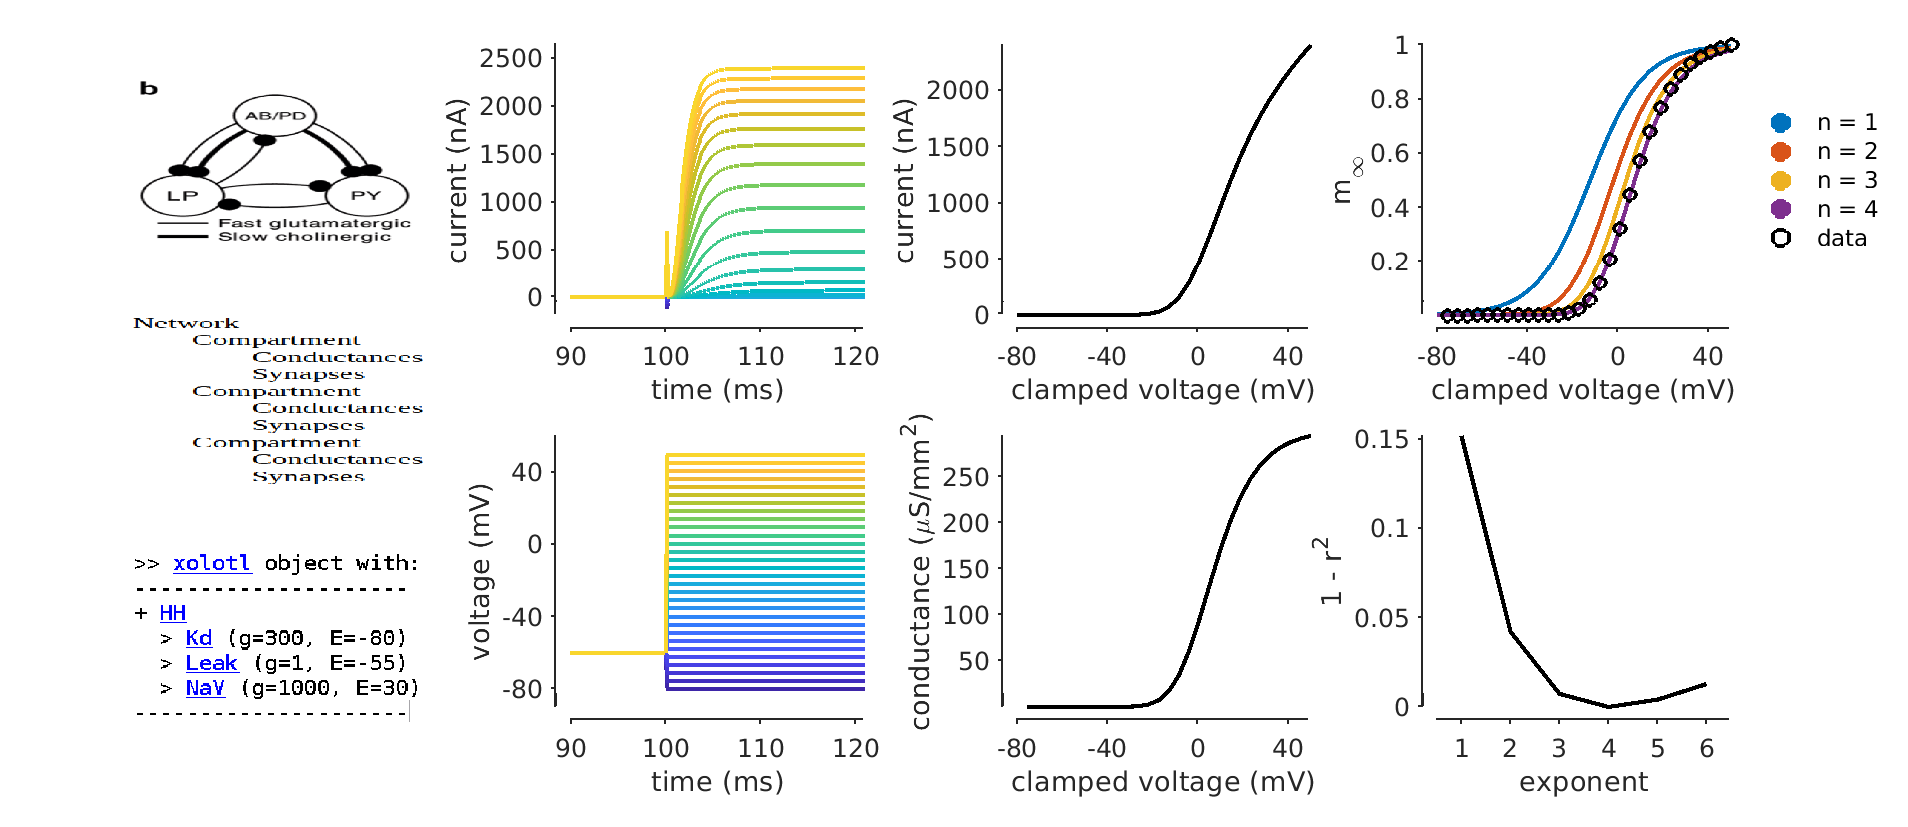
\includegraphics[width=1.0\linewidth]{gfx/figure_clamp}
	\caption{Simulating a voltage-clamp experiment. (A) Cartoon of a cell with delayed rectifier potassium conductance (\cite{liuModelNeuronActivitydependent1998} with experimentally-fixed voltage. (B) Structure of \texttt{xolotl} object in A. (C) Code snippet depicting integration under voltage clamp. (D-E) Current response to steps in voltage from a holding potential of $V_m = -60$ mV. (F) Current-voltage relation of the steady-state current ($t = 400$ ms) indicating a reversal potential of $E = -80$ mV and no inactivation. (G) Conductance-voltage relation at steady-state takes the form of a sigmoid. (H) Sigmoids $m$ fit to the model as $m^n$ data indicating that $n=4$ is the best fit. (I) Goodness of fit vs. exponent $n$, suggesting $n=4$ as the best fit to the data.}
	\label{fig:figureclamp}
\end{figure}

\begin{figure}
	\centering
	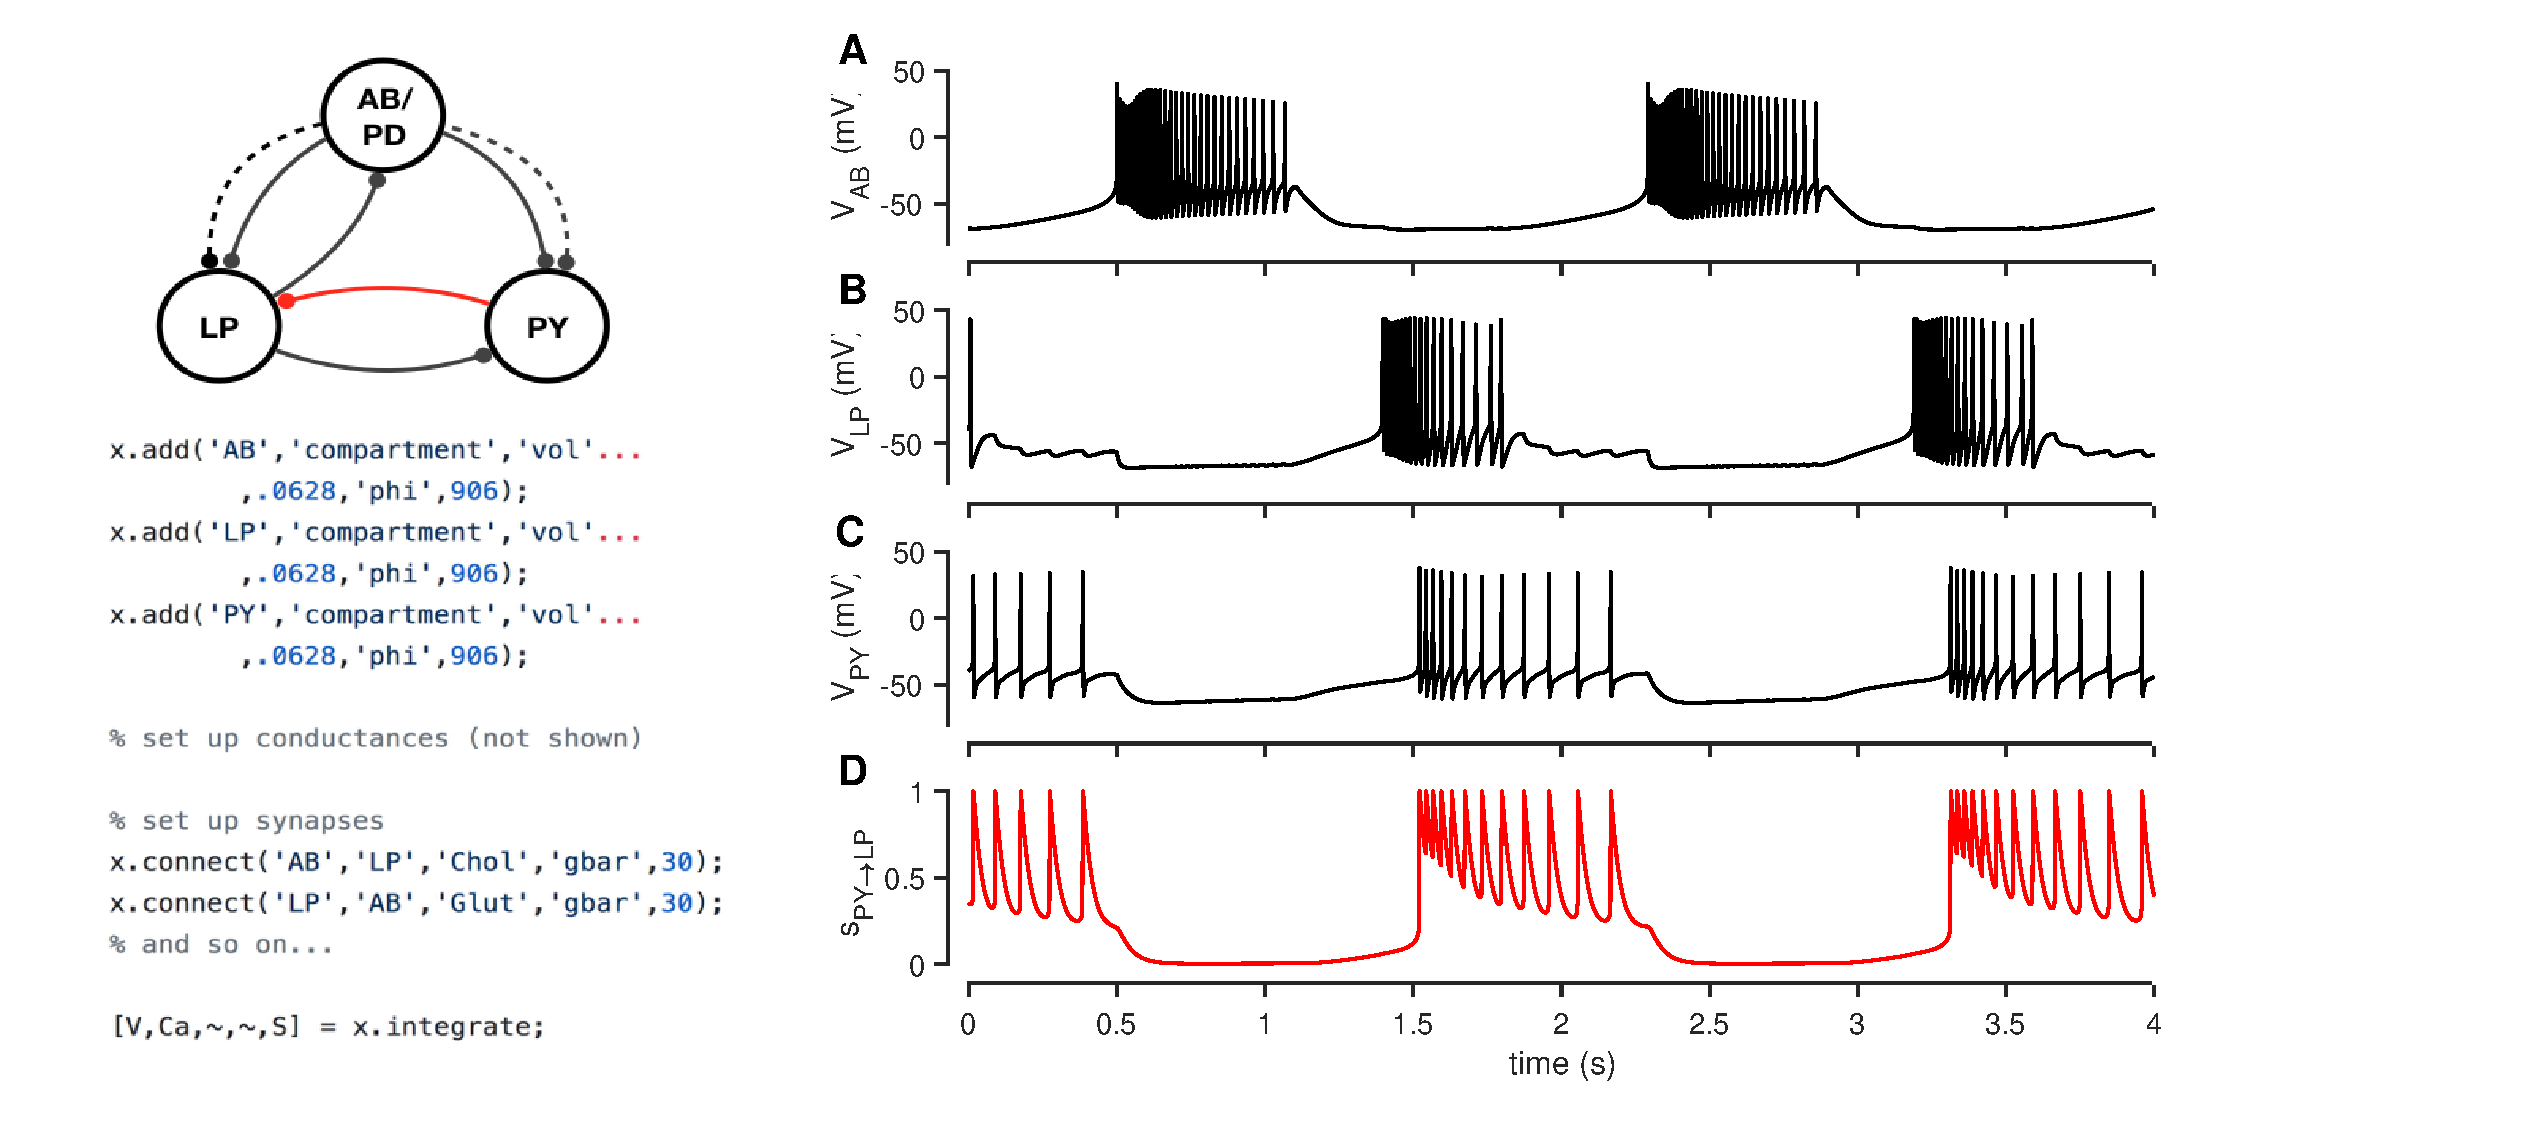
\includegraphics[width=1.0\linewidth]{gfx/figure_network}
	\caption{Simulating a network of conductance-based model neurons. (A) Diagram of a network model of the pyloric rhythm in the crustacean stomatogastric ganglion (Prinz \textit{et al.} 2004). (B) Each neuron is modeled as a single compartment with 7-8 intrinsic conductances and 1-3 post-synaptic conductances. (C) \texttt{xolotl} implements conductances as fields of compartments and synapses as connections between compartments. (D-F) Simulated voltage trace of a model network for the three compartments. (G) Time series of synaptic currents in the simulated network can be obtained from the integration.}
	\label{fig:figurenetwork}
\end{figure}

\begin{figure}
	\centering
	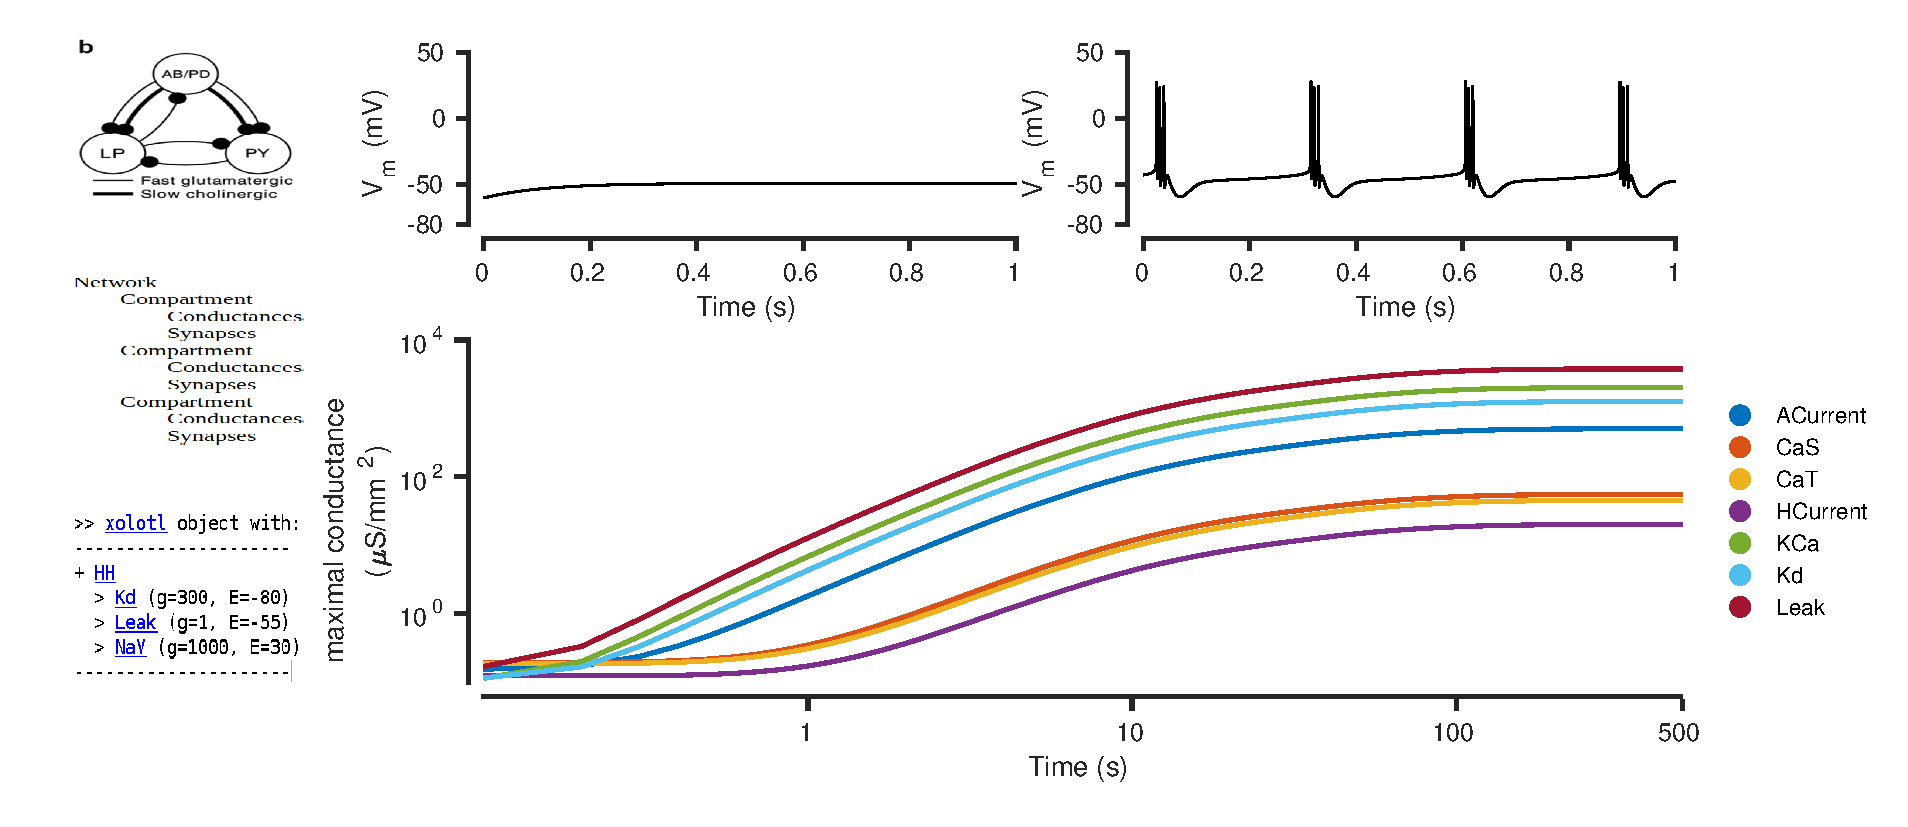
\includegraphics[width=1.0\linewidth]{gfx/figure_integral_control}
	\caption{Simulating neurons under homeostatic regulation. (A) Cartoon of a model neuron (\cite{liuModelNeuronActivitydependent1998} with integral control (\cite{olearyCorrelationsIonChannel2013}. (B) Hierarchical structure of a neuronal network considers controllers as components of compartments which act on conductances. (C) \texttt{xolotl} implements controllers as properties of conductances and synapses. (D) Calcium sensors change maximal conductances to move a neuron from quiescence to a bursting state. (E) Voltage trace shows regular bursting activity after integral control.}
	\label{fig:figureintegralcontrol}
\end{figure}

\begin{figure}
	\centering
	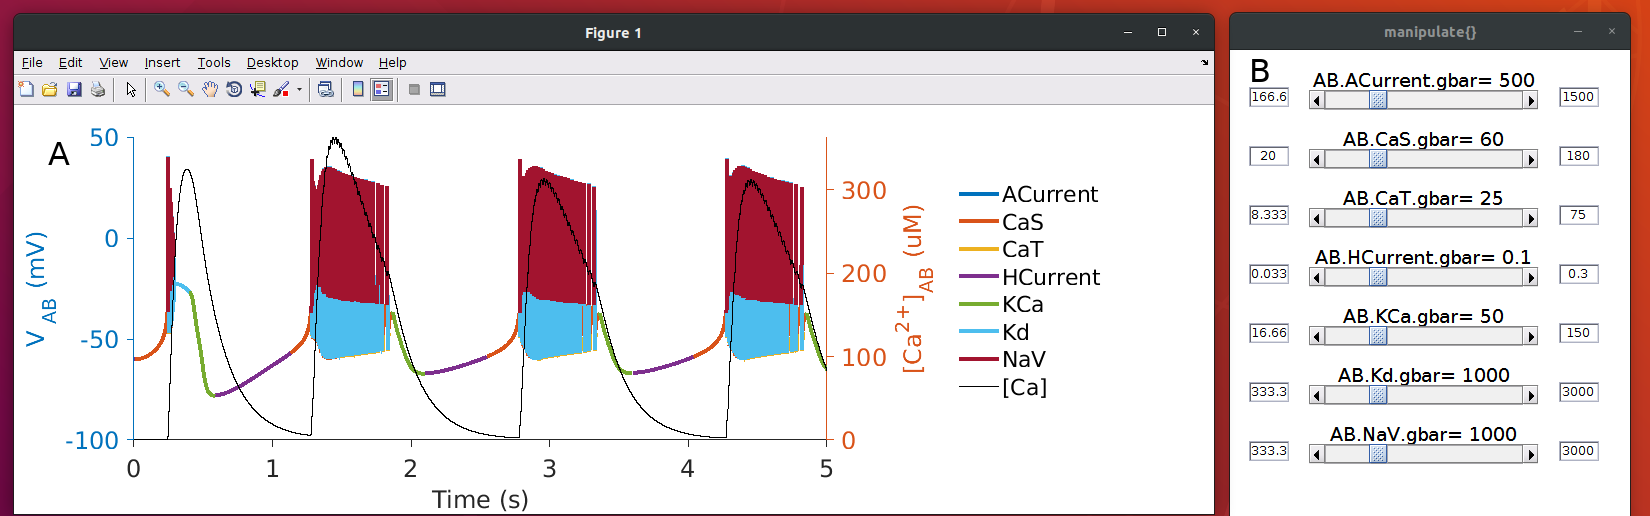
\includegraphics[width=1.0\linewidth]{gfx/puppeteer_screenshot}
	\caption{Using the GUI to manipulate neuron parameters. (A) Real-time output of the \texttt{plot} function displaying voltage (colored) and intracellular calcium (black) traces of a bursting neuron model (\cite{prinzAlternativeHandtuningConductancebased2003, prinzSimilarNetworkActivity2004}. Colors indicate the dominant current. (B) Sliders control the maximal conductances, which updates on the figure.}
	\label{fig:puppeteerscreenshot}
\end{figure}


\begin{figure}
	\centering
	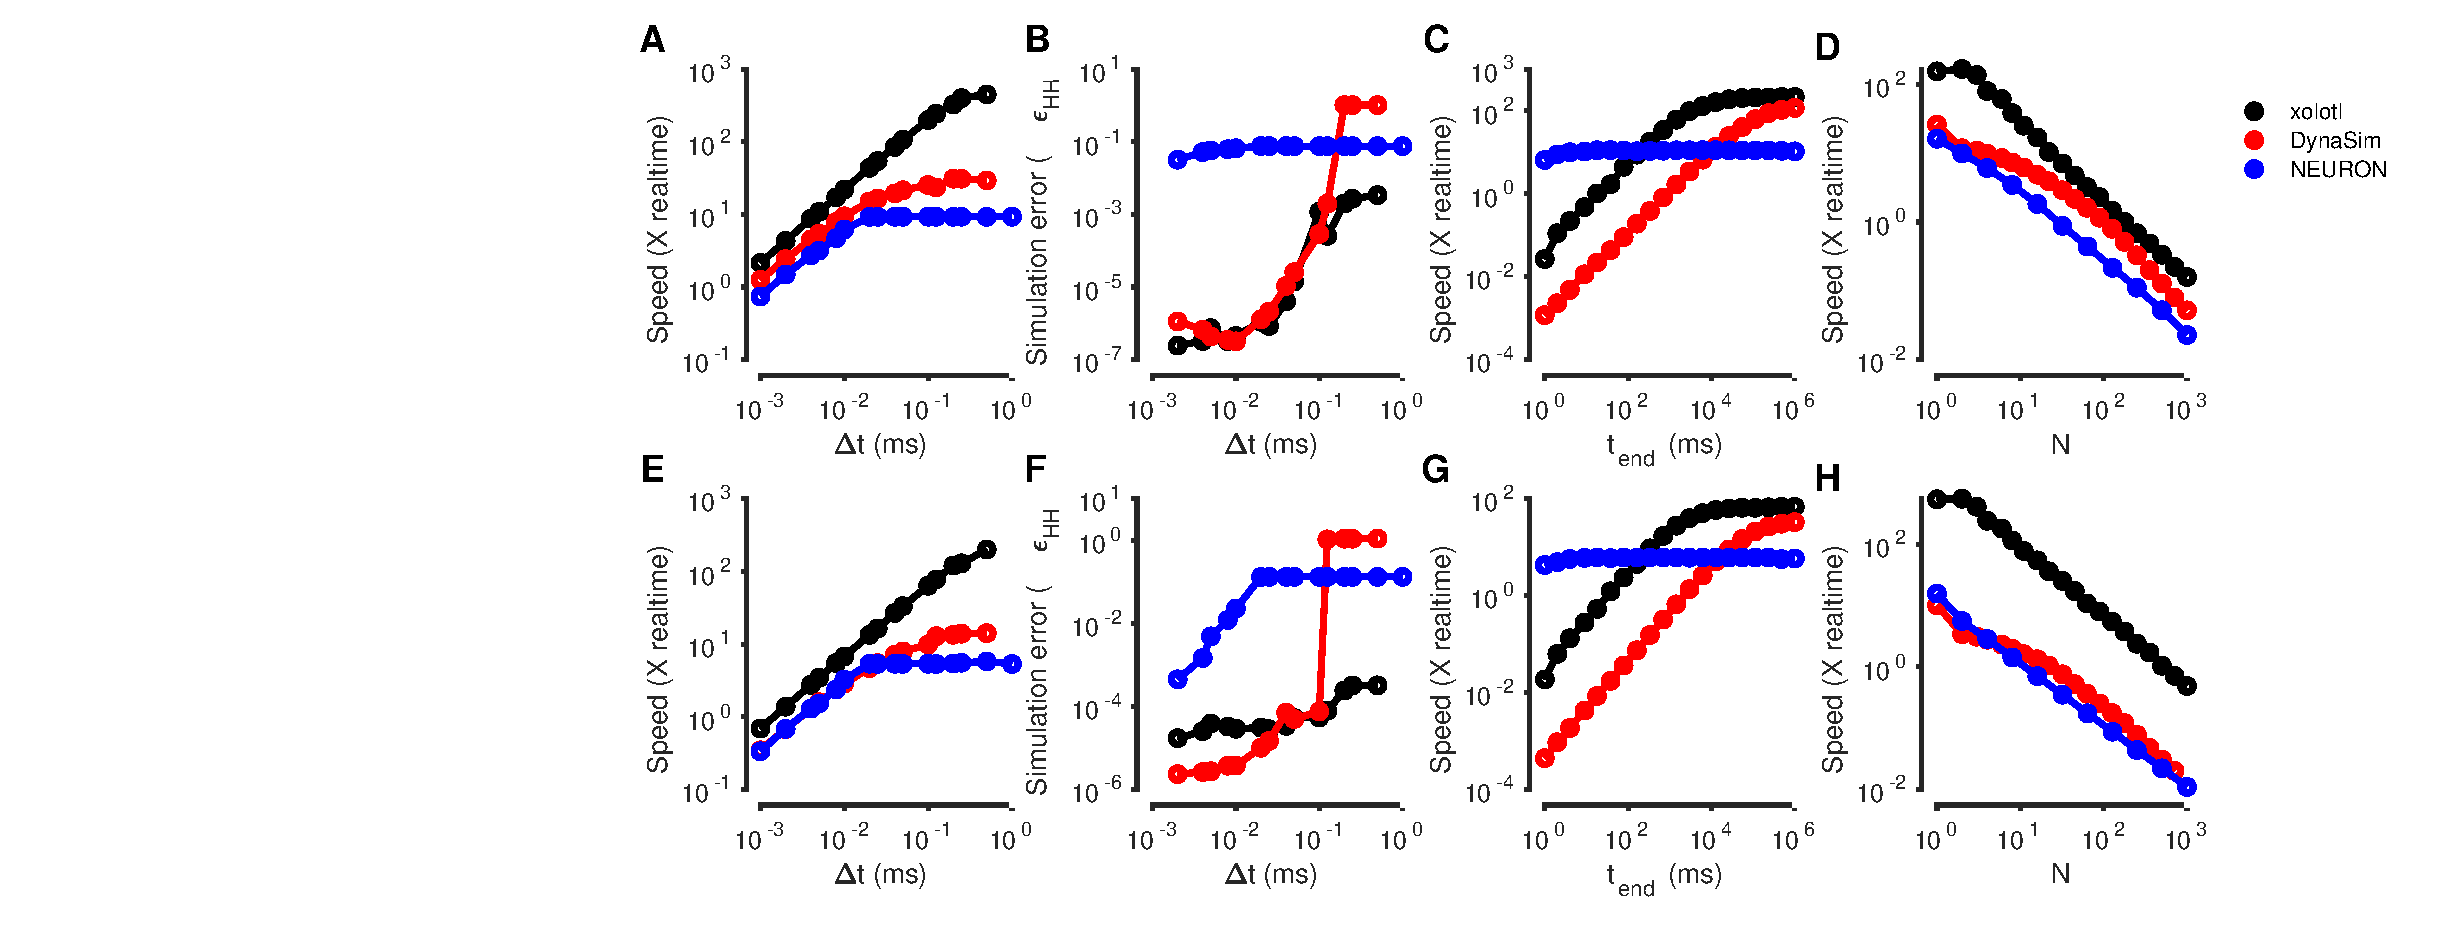
\includegraphics[width=1.0\linewidth]{gfx/figure_benchmark}
	\caption{\texttt{xolotl} benchmarked against \texttt{DynaSim} and \texttt{NEURON}. (A) Ratio of 'simulated' time to runtime (speed factor) and accuracy, measured by spike train coincidence plotted against decreasing time-resolution. (B) Speed factor for models at increasing simulation times. (C) Speed factor over number of compartments.}
	\label{fig:figurebenchmark}
\end{figure}


\end{document}